\documentclass[1p]{elsarticle_modified}
%\bibliographystyle{elsarticle-num}

%\usepackage[colorlinks]{hyperref}
%\usepackage{abbrmath_seonhwa} %\Abb, \Ascr, \Acal ,\Abf, \Afrak
\usepackage{amsfonts}
\usepackage{amssymb}
\usepackage{amsmath}
\usepackage{amsthm}
\usepackage{scalefnt}
\usepackage{amsbsy}
\usepackage{kotex}
\usepackage{caption}
\usepackage{subfig}
\usepackage{color}
\usepackage{graphicx}
\usepackage{xcolor} %% white, black, red, green, blue, cyan, magenta, yellow
\usepackage{float}
\usepackage{setspace}
\usepackage{hyperref}

\usepackage{tikz}
\usetikzlibrary{arrows}

\usepackage{multirow}
\usepackage{array} % fixed length table
\usepackage{hhline}

%%%%%%%%%%%%%%%%%%%%%
\makeatletter
\renewcommand*\env@matrix[1][\arraystretch]{%
	\edef\arraystretch{#1}%
	\hskip -\arraycolsep
	\let\@ifnextchar\new@ifnextchar
	\array{*\c@MaxMatrixCols c}}
\makeatother %https://tex.stackexchange.com/questions/14071/how-can-i-increase-the-line-spacing-in-a-matrix
%%%%%%%%%%%%%%%

\usepackage[normalem]{ulem}

\newcommand{\msout}[1]{\ifmmode\text{\sout{\ensuremath{#1}}}\else\sout{#1}\fi}
%SOURCE: \msout is \stkout macro in https://tex.stackexchange.com/questions/20609/strikeout-in-math-mode

\newcommand{\cancel}[1]{
	\ifmmode
	{\color{red}\msout{#1}}
	\else
	{\color{red}\sout{#1}}
	\fi
}

\newcommand{\add}[1]{
	{\color{blue}\uwave{#1}}
}

\newcommand{\replace}[2]{
	\ifmmode
	{\color{red}\msout{#1}}{\color{blue}\uwave{#2}}
	\else
	{\color{red}\sout{#1}}{\color{blue}\uwave{#2}}
	\fi
}

\newcommand{\Sol}{\mathcal{S}} %segment
\newcommand{\D}{D} %diagram
\newcommand{\A}{\mathcal{A}} %arc


%%%%%%%%%%%%%%%%%%%%%%%%%%%%%5 test

\def\sl{\operatorname{\textup{SL}}(2,\Cbb)}
\def\psl{\operatorname{\textup{PSL}}(2,\Cbb)}
\def\quan{\mkern 1mu \triangleright \mkern 1mu}

\theoremstyle{definition}
\newtheorem{thm}{Theorem}[section]
\newtheorem{prop}[thm]{Proposition}
\newtheorem{lem}[thm]{Lemma}
\newtheorem{ques}[thm]{Question}
\newtheorem{cor}[thm]{Corollary}
\newtheorem{defn}[thm]{Definition}
\newtheorem{exam}[thm]{Example}
\newtheorem{rmk}[thm]{Remark}
\newtheorem{alg}[thm]{Algorithm}

\newcommand{\I}{\sqrt{-1}}
\begin{document}

%\begin{frontmatter}
%
%\title{Boundary parabolic representations of knots up to 8 crossings}
%
%%% Group authors per affiliation:
%\author{Yunhi Cho} 
%\address{Department of Mathematics, University of Seoul, Seoul, Korea}
%\ead{yhcho@uos.ac.kr}
%
%
%\author{Seonhwa Kim} %\fnref{s_kim}}
%\address{Center for Geometry and Physics, Institute for Basic Science, Pohang, 37673, Korea}
%\ead{ryeona17@ibs.re.kr}
%
%\author{Hyuk Kim}
%\address{Department of Mathematical Sciences, Seoul National University, Seoul 08826, Korea}
%\ead{hyukkim@snu.ac.kr}
%
%\author{Seokbeom Yoon}
%\address{Department of Mathematical Sciences, Seoul National University, Seoul, 08826,  Korea}
%\ead{sbyoon15@snu.ac.kr}
%
%\begin{abstract}
%We find all boundary parabolic representation of knots up to 8 crossings.
%
%\end{abstract}
%\begin{keyword}
%    \MSC[2010] 57M25 
%\end{keyword}
%
%\end{frontmatter}

%\linenumbers
%\tableofcontents
%
\newcommand\colored[1]{\textcolor{white}{\rule[-0.35ex]{0.8em}{1.4ex}}\kern-0.8em\color{red} #1}%
%\newcommand\colored[1]{\textcolor{white}{ #1}\kern-2.17ex	\textcolor{white}{ #1}\kern-1.81ex	\textcolor{white}{ #1}\kern-2.15ex\color{red}#1	}

{\Large $\underline{11n_{144}~(K11n_{144})}$}

\setlength{\tabcolsep}{10pt}
\renewcommand{\arraystretch}{1.6}
\vspace{1cm}\begin{tabular}{m{100pt}>{\centering\arraybackslash}m{274pt}}
\multirow{5}{120pt}{
	\centering
	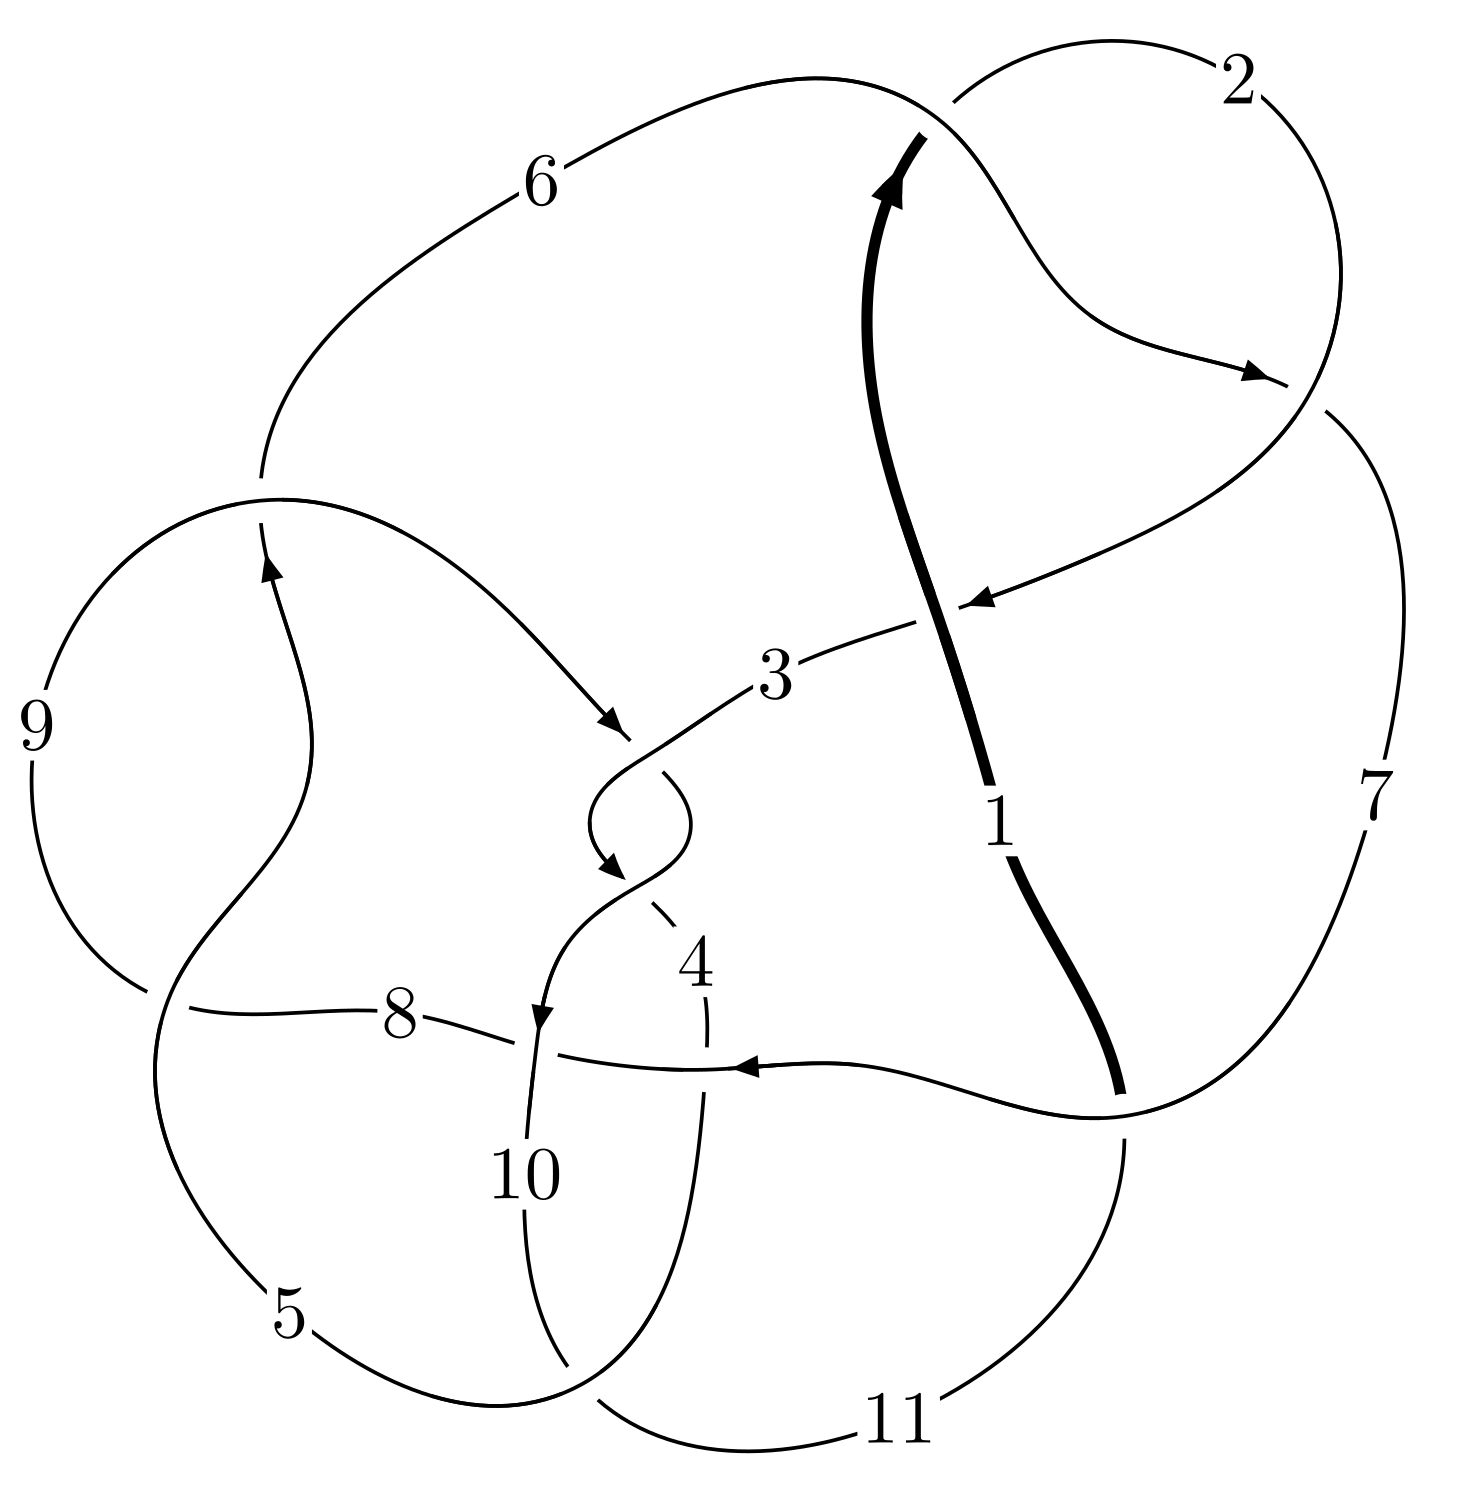
\includegraphics[width=112pt]{../../../GIT/diagram.site/Diagrams/png/760_11n_144.png}\\
\ \ \ A knot diagram\footnotemark}&
\allowdisplaybreaks
\textbf{Linearized knot diagam} \\
\cline{2-2}
 &
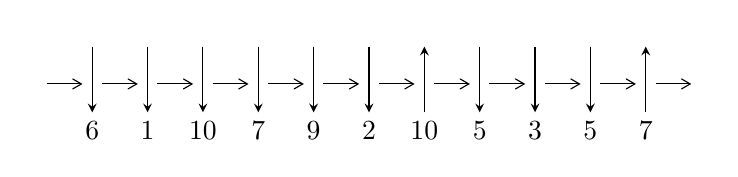
\begin{tikzpicture}[x=20pt, y=17pt]
	% nodes
	\node (C0) at (0, 0) {};
	\node (C1) at (1, 0) {};
	\node (C1U) at (1, +1) {};
	\node (C1D) at (1, -1) {6};

	\node (C2) at (2, 0) {};
	\node (C2U) at (2, +1) {};
	\node (C2D) at (2, -1) {1};

	\node (C3) at (3, 0) {};
	\node (C3U) at (3, +1) {};
	\node (C3D) at (3, -1) {10};

	\node (C4) at (4, 0) {};
	\node (C4U) at (4, +1) {};
	\node (C4D) at (4, -1) {7};

	\node (C5) at (5, 0) {};
	\node (C5U) at (5, +1) {};
	\node (C5D) at (5, -1) {9};

	\node (C6) at (6, 0) {};
	\node (C6U) at (6, +1) {};
	\node (C6D) at (6, -1) {2};

	\node (C7) at (7, 0) {};
	\node (C7U) at (7, +1) {};
	\node (C7D) at (7, -1) {10};

	\node (C8) at (8, 0) {};
	\node (C8U) at (8, +1) {};
	\node (C8D) at (8, -1) {5};

	\node (C9) at (9, 0) {};
	\node (C9U) at (9, +1) {};
	\node (C9D) at (9, -1) {3};

	\node (C10) at (10, 0) {};
	\node (C10U) at (10, +1) {};
	\node (C10D) at (10, -1) {5};

	\node (C11) at (11, 0) {};
	\node (C11U) at (11, +1) {};
	\node (C11D) at (11, -1) {7};
	\node (C12) at (12, 0) {};

	% arrows
	\draw[->,>={angle 60}]
	(C0) edge (C1) (C1) edge (C2) (C2) edge (C3) (C3) edge (C4) (C4) edge (C5) (C5) edge (C6) (C6) edge (C7) (C7) edge (C8) (C8) edge (C9) (C9) edge (C10) (C10) edge (C11) (C11) edge (C12) ;	\draw[->,>=stealth]
	(C1U) edge (C1D) (C2U) edge (C2D) (C3U) edge (C3D) (C4U) edge (C4D) (C5U) edge (C5D) (C6U) edge (C6D) (C7D) edge (C7U) (C8U) edge (C8D) (C9U) edge (C9D) (C10U) edge (C10D) (C11D) edge (C11U) ;
	\end{tikzpicture} \\
\hhline{~~} \\& 
\textbf{Solving Sequence} \\ \cline{2-2} 
 &
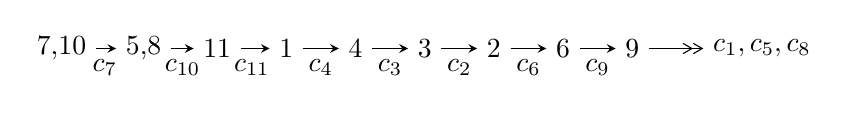
\begin{tikzpicture}[x=25pt, y=7pt]
	% node
	\node (A0) at (-1/8, 0) {7,10};
	\node (A1) at (17/16, 0) {5,8};
	\node (A2) at (17/8, 0) {11};
	\node (A3) at (25/8, 0) {1};
	\node (A4) at (33/8, 0) {4};
	\node (A5) at (41/8, 0) {3};
	\node (A6) at (49/8, 0) {2};
	\node (A7) at (57/8, 0) {6};
	\node (A8) at (65/8, 0) {9};
	\node (C1) at (1/2, -1) {$c_{7}$};
	\node (C2) at (13/8, -1) {$c_{10}$};
	\node (C3) at (21/8, -1) {$c_{11}$};
	\node (C4) at (29/8, -1) {$c_{4}$};
	\node (C5) at (37/8, -1) {$c_{3}$};
	\node (C6) at (45/8, -1) {$c_{2}$};
	\node (C7) at (53/8, -1) {$c_{6}$};
	\node (C8) at (61/8, -1) {$c_{9}$};
	\node (A9) at (10, 0) {$c_{1},c_{5},c_{8}$};

	% edge
	\draw[->,>=stealth]	
	(A0) edge (A1) (A1) edge (A2) (A2) edge (A3) (A3) edge (A4) (A4) edge (A5) (A5) edge (A6) (A6) edge (A7) (A7) edge (A8) ;
	\draw[->>,>={angle 60}]	
	(A8) edge (A9);
\end{tikzpicture} \\ 

\end{tabular} \\

\footnotetext{
The image of knot diagram is generated by the software ``\textbf{Draw programme}" developed by Andrew Bartholomew(\url{http://www.layer8.co.uk/maths/draw/index.htm\#Running-draw}), where we modified some parts for our purpose(\url{https://github.com/CATsTAILs/LinksPainter}).
}\phantom \\ \newline 
\centering \textbf{Ideals for irreducible components\footnotemark of $X_{\text{par}}$} 
 
\begin{align*}
I^u_{1}&=\langle 
19 u^{18}-215 u^{17}+\cdots+32 b+896,\;-14 u^{18}+191 u^{17}+\cdots+32 a-1760,\\
\phantom{I^u_{1}}&\phantom{= \langle  }u^{19}-15 u^{18}+\cdots+544 u-64\rangle \\
I^u_{2}&=\langle 
-25111 a^{11} u+473518 a^{10} u+\cdots-96138 a-81801,\;a^{11} u-6 a^{10} u+\cdots-155 a+167,\;u^2+u-1\rangle \\
I^u_{3}&=\langle 
3 u^{10}+8 u^9+u^8-3 u^7+8 u^6- u^5- u^4+3 u^3-9 u^2+b+u-1,\\
\phantom{I^u_{3}}&\phantom{= \langle  }- u^{10}- u^9+4 u^8+u^7-5 u^6+5 u^5-2 u^3+5 u^2+a-5 u+1,\\
\phantom{I^u_{3}}&\phantom{= \langle  }u^{11}+4 u^{10}+4 u^9+2 u^7+3 u^6- u^5+u^4-2 u^3-4 u^2-1\rangle \\
\\
\end{align*}
\raggedright * 3 irreducible components of $\dim_{\mathbb{C}}=0$, with total 54 representations.\\
\footnotetext{All coefficients of polynomials are rational numbers. But the coefficients are sometimes approximated in decimal forms when there is not enough margin.}
\newpage
\renewcommand{\arraystretch}{1}
\centering \section*{I. $I^u_{1}= \langle 19 u^{18}-215 u^{17}+\cdots+32 b+896,\;-14 u^{18}+191 u^{17}+\cdots+32 a-1760,\;u^{19}-15 u^{18}+\cdots+544 u-64 \rangle$}
\flushleft \textbf{(i) Arc colorings}\\
\begin{tabular}{m{7pt} m{180pt} m{7pt} m{180pt} }
\flushright $a_{7}=$&$\begin{pmatrix}1\\0\end{pmatrix}$ \\
\flushright $a_{10}=$&$\begin{pmatrix}0\\u\end{pmatrix}$ \\
\flushright $a_{5}=$&$\begin{pmatrix}\frac{7}{16} u^{18}-\frac{191}{32} u^{17}+\cdots-\frac{743}{2} u+55\\-\frac{19}{32} u^{18}+\frac{215}{32} u^{17}+\cdots+183 u-28\end{pmatrix}$ \\
\flushright $a_{8}=$&$\begin{pmatrix}1\\- u^2\end{pmatrix}$ \\
\flushright $a_{11}=$&$\begin{pmatrix}-\frac{63}{64} u^{18}+\frac{883}{64} u^{17}+\cdots+\frac{1901}{4} u-64\\\frac{31}{32} u^{18}-\frac{435}{32} u^{17}+\cdots-\frac{941}{2} u+63\end{pmatrix}$ \\
\flushright $a_{1}=$&$\begin{pmatrix}-\frac{1}{64} u^{18}+\frac{13}{64} u^{17}+\cdots+\frac{19}{4} u-1\\\frac{31}{32} u^{18}-\frac{435}{32} u^{17}+\cdots-\frac{941}{2} u+63\end{pmatrix}$ \\
\flushright $a_{4}=$&$\begin{pmatrix}-\frac{5}{32} u^{18}+\frac{3}{4} u^{17}+\cdots-\frac{377}{2} u+27\\-\frac{19}{32} u^{18}+\frac{215}{32} u^{17}+\cdots+183 u-28\end{pmatrix}$ \\
\flushright $a_{3}=$&$\begin{pmatrix}-\frac{5}{32} u^{18}+\frac{3}{4} u^{17}+\cdots-\frac{377}{2} u+27\\\frac{115}{32} u^{18}-\frac{1551}{32} u^{17}+\cdots-674 u+74\end{pmatrix}$ \\
\flushright $a_{2}=$&$\begin{pmatrix}\frac{307}{64} u^{18}-\frac{3931}{64} u^{17}+\cdots-\frac{3381}{4} u+100\\-\frac{177}{32} u^{18}+\frac{2313}{32} u^{17}+\cdots+\frac{2457}{2} u-149\end{pmatrix}$ \\
\flushright $a_{6}=$&$\begin{pmatrix}-\frac{137}{64} u^{18}+\frac{1597}{64} u^{17}+\cdots-61 u+\frac{37}{2}\\\frac{339}{32} u^{18}-\frac{4473}{32} u^{17}+\cdots-2502 u+303\end{pmatrix}$ \\
\flushright $a_{9}=$&$\begin{pmatrix}-0.0156250 u^{18}+0.203125 u^{17}+\cdots-10.3750 u^{2}+3.75000 u\\\frac{1}{32} u^{18}-\frac{13}{32} u^{17}+\cdots-\frac{15}{2} u+1\end{pmatrix}$\\ \flushright $a_{9}=$&$\begin{pmatrix}-0.0156250 u^{18}+0.203125 u^{17}+\cdots-10.3750 u^{2}+3.75000 u\\\frac{1}{32} u^{18}-\frac{13}{32} u^{17}+\cdots-\frac{15}{2} u+1\end{pmatrix}$\\&\end{tabular}
\flushleft \textbf{(ii) Obstruction class $= -1$}\\~\\
\flushleft \textbf{(iii) Cusp Shapes $= -\frac{107}{8} u^{18}+\frac{1433}{8} u^{17}+\cdots+4122 u-534$}\\~\\
\newpage\renewcommand{\arraystretch}{1}
\flushleft \textbf{(iv) u-Polynomials at the component}\newline \\
\begin{tabular}{m{50pt}|m{274pt}}
Crossings & \hspace{64pt}u-Polynomials at each crossing \\
\hline $$\begin{aligned}c_{1},c_{6}\end{aligned}$$&$\begin{aligned}
&u^{19}-5 u^{18}+\cdots-14 u+4
\end{aligned}$\\
\hline $$\begin{aligned}c_{2}\end{aligned}$$&$\begin{aligned}
&u^{19}+9 u^{18}+\cdots+44 u+16
\end{aligned}$\\
\hline $$\begin{aligned}c_{3},c_{5},c_{8}\\c_{9}\end{aligned}$$&$\begin{aligned}
&u^{19}+u^{18}+\cdots+4 u+1
\end{aligned}$\\
\hline $$\begin{aligned}c_{4},c_{10}\end{aligned}$$&$\begin{aligned}
&u^{19}+15 u^{17}+\cdots+3 u+1
\end{aligned}$\\
\hline $$\begin{aligned}c_{7}\end{aligned}$$&$\begin{aligned}
&u^{19}+15 u^{18}+\cdots+544 u+64
\end{aligned}$\\
\hline $$\begin{aligned}c_{11}\end{aligned}$$&$\begin{aligned}
&u^{19}-15 u^{18}+\cdots-990 u+196
\end{aligned}$\\
\hline
\end{tabular}\\~\\
\newpage\renewcommand{\arraystretch}{1}
\flushleft \textbf{(v) Riley Polynomials at the component}\newline \\
\begin{tabular}{m{50pt}|m{274pt}}
Crossings & \hspace{64pt}Riley Polynomials at each crossing \\
\hline $$\begin{aligned}c_{1},c_{6}\end{aligned}$$&$\begin{aligned}
&y^{19}-9 y^{18}+\cdots+44 y-16
\end{aligned}$\\
\hline $$\begin{aligned}c_{2}\end{aligned}$$&$\begin{aligned}
&y^{19}+3 y^{18}+\cdots+2288 y-256
\end{aligned}$\\
\hline $$\begin{aligned}c_{3},c_{5},c_{8}\\c_{9}\end{aligned}$$&$\begin{aligned}
&y^{19}-9 y^{18}+\cdots+12 y-1
\end{aligned}$\\
\hline $$\begin{aligned}c_{4},c_{10}\end{aligned}$$&$\begin{aligned}
&y^{19}+30 y^{18}+\cdots-25 y-1
\end{aligned}$\\
\hline $$\begin{aligned}c_{7}\end{aligned}$$&$\begin{aligned}
&y^{19}-11 y^{18}+\cdots+95232 y-4096
\end{aligned}$\\
\hline $$\begin{aligned}c_{11}\end{aligned}$$&$\begin{aligned}
&y^{19}+3 y^{18}+\cdots+237260 y-38416
\end{aligned}$\\
\hline
\end{tabular}\\~\\
\newpage\flushleft \textbf{(vi) Complex Volumes and Cusp Shapes}
$$\begin{array}{c|c|c}  
\text{Solutions to }I^u_{1}& \I (\text{vol} + \sqrt{-1}CS) & \text{Cusp shape}\\
 \hline 
\begin{aligned}
u &= \phantom{-}0.068838 + 1.152610 I \\
a &= \phantom{-}0.509367 - 0.020838 I \\
b &= -0.059082 - 0.585665 I\end{aligned}
 & -1.40681 - 1.74274 I & -5.94701 + 3.80028 I \\ \hline\begin{aligned}
u &= \phantom{-}0.068838 - 1.152610 I \\
a &= \phantom{-}0.509367 + 0.020838 I \\
b &= -0.059082 + 0.585665 I\end{aligned}
 & -1.40681 + 1.74274 I & -5.94701 - 3.80028 I \\ \hline\begin{aligned}
u &= -0.655172 + 0.270735 I \\
a &= \phantom{-}0.180740 - 0.531477 I \\
b &= -0.025474 - 0.397141 I\end{aligned}
 & \phantom{-}1.11792 - 1.95845 I & -4.20644 + 5.46350 I \\ \hline\begin{aligned}
u &= -0.655172 - 0.270735 I \\
a &= \phantom{-}0.180740 + 0.531477 I \\
b &= -0.025474 + 0.397141 I\end{aligned}
 & \phantom{-}1.11792 + 1.95845 I & -4.20644 - 5.46350 I \\ \hline\begin{aligned}
u &= \phantom{-}1.244400 + 0.434239 I \\
a &= \phantom{-}0.558407 + 1.198070 I \\
b &= -0.17463 - 1.73336 I\end{aligned}
 & \phantom{-}5.25710 - 1.54392 I & -8.61355 - 2.51619 I \\ \hline\begin{aligned}
u &= \phantom{-}1.244400 - 0.434239 I \\
a &= \phantom{-}0.558407 - 1.198070 I \\
b &= -0.17463 + 1.73336 I\end{aligned}
 & \phantom{-}5.25710 + 1.54392 I & -8.61355 + 2.51619 I \\ \hline\begin{aligned}
u &= \phantom{-}0.525160 + 1.295010 I \\
a &= -0.477990 - 0.189359 I \\
b &= \phantom{-}0.005800 + 0.718444 I\end{aligned}
 & -5.26090 + 2.36693 I & -9.94736 - 1.06990 I \\ \hline\begin{aligned}
u &= \phantom{-}0.525160 - 1.295010 I \\
a &= -0.477990 + 0.189359 I \\
b &= \phantom{-}0.005800 - 0.718444 I\end{aligned}
 & -5.26090 - 2.36693 I & -9.94736 + 1.06990 I \\ \hline\begin{aligned}
u &= \phantom{-}1.37929 + 0.44772 I \\
a &= -0.340635 - 1.191440 I \\
b &= -0.06359 + 1.79584 I\end{aligned}
 & \phantom{-}6.12748 + 4.38921 I & -5.85287 - 6.32556 I \\ \hline\begin{aligned}
u &= \phantom{-}1.37929 - 0.44772 I \\
a &= -0.340635 + 1.191440 I \\
b &= -0.06359 - 1.79584 I\end{aligned}
 & \phantom{-}6.12748 - 4.38921 I & -5.85287 + 6.32556 I\\
 \hline 
 \end{array}$$\newpage$$\begin{array}{c|c|c}  
\text{Solutions to }I^u_{1}& \I (\text{vol} + \sqrt{-1}CS) & \text{Cusp shape}\\
 \hline 
\begin{aligned}
u &= -0.07036 + 1.50415 I \\
a &= -0.374863 + 0.006918 I \\
b &= -0.015967 + 0.564338 I\end{aligned}
 & -4.57325 - 6.41400 I & -8.03245 + 7.39287 I \\ \hline\begin{aligned}
u &= -0.07036 - 1.50415 I \\
a &= -0.374863 - 0.006918 I \\
b &= -0.015967 - 0.564338 I\end{aligned}
 & -4.57325 + 6.41400 I & -8.03245 - 7.39287 I \\ \hline\begin{aligned}
u &= \phantom{-}1.57100 + 0.65066 I \\
a &= \phantom{-}0.118849 + 0.926036 I \\
b &= \phantom{-}0.41582 - 1.53213 I\end{aligned}
 & -1.49409 + 5.07243 I & -11.25567 - 3.29320 I \\ \hline\begin{aligned}
u &= \phantom{-}1.57100 - 0.65066 I \\
a &= \phantom{-}0.118849 - 0.926036 I \\
b &= \phantom{-}0.41582 + 1.53213 I\end{aligned}
 & -1.49409 - 5.07243 I & -11.25567 + 3.29320 I \\ \hline\begin{aligned}
u &= \phantom{-}1.63033 + 0.51703 I \\
a &= -0.023365 - 1.061980 I \\
b &= -0.51099 + 1.74346 I\end{aligned}
 & \phantom{-}4.00668 + 8.26944 I & -5.84435 - 4.36564 I \\ \hline\begin{aligned}
u &= \phantom{-}1.63033 - 0.51703 I \\
a &= -0.023365 + 1.061980 I \\
b &= -0.51099 - 1.74346 I\end{aligned}
 & \phantom{-}4.00668 - 8.26944 I & -5.84435 + 4.36564 I \\ \hline\begin{aligned}
u &= \phantom{-}1.69551 + 0.51970 I \\
a &= -0.052766 + 1.037060 I \\
b &= \phantom{-}0.62842 - 1.73093 I\end{aligned}
 & \phantom{-}1.54987 + 13.80210 I & -8.55217 - 7.85507 I \\ \hline\begin{aligned}
u &= \phantom{-}1.69551 - 0.51970 I \\
a &= -0.052766 - 1.037060 I \\
b &= \phantom{-}0.62842 + 1.73093 I\end{aligned}
 & \phantom{-}1.54987 - 13.80210 I & -8.55217 + 7.85507 I \\ \hline\begin{aligned}
u &= \phantom{-}0.222014\phantom{ +0.000000I} \\
a &= \phantom{-}1.80451\phantom{ +0.000000I} \\
b &= -0.400627\phantom{ +0.000000I}\end{aligned}
 & -0.778408\phantom{ +0.000000I} & -13.4960\phantom{ +0.000000I}\\
 \hline 
 \end{array}$$\newpage\newpage\renewcommand{\arraystretch}{1}
\centering \section*{II. $I^u_{2}= \langle -2.51\times10^{4} a^{11} u+4.74\times10^{5} a^{10} u+\cdots-9.61\times10^{4} a-8.18\times10^{4},\;a^{11} u-6 a^{10} u+\cdots-155 a+167,\;u^2+u-1 \rangle$}
\flushleft \textbf{(i) Arc colorings}\\
\begin{tabular}{m{7pt} m{180pt} m{7pt} m{180pt} }
\flushright $a_{7}=$&$\begin{pmatrix}1\\0\end{pmatrix}$ \\
\flushright $a_{10}=$&$\begin{pmatrix}0\\u\end{pmatrix}$ \\
\flushright $a_{5}=$&$\begin{pmatrix}a\\1.13517 a^{11} u-21.4058 a^{10} u+\cdots+4.34601 a+3.69789\end{pmatrix}$ \\
\flushright $a_{8}=$&$\begin{pmatrix}1\\u-1\end{pmatrix}$ \\
\flushright $a_{11}=$&$\begin{pmatrix}- a^2 u\\-35.3361 a^{11} u-18.9502 a^{10} u+\cdots+8.81063 a+0.563175\end{pmatrix}$ \\
\flushright $a_{1}=$&$\begin{pmatrix}-35.3361 a^{11} u-18.9502 a^{10} u+\cdots+8.81063 a+0.563175\\-35.3361 a^{11} u-18.9502 a^{10} u+\cdots+8.81063 a+0.563175\end{pmatrix}$ \\
\flushright $a_{4}=$&$\begin{pmatrix}1.13517 a^{11} u-21.4058 a^{10} u+\cdots+5.34601 a+3.69789\\1.13517 a^{11} u-21.4058 a^{10} u+\cdots+4.34601 a+3.69789\end{pmatrix}$ \\
\flushright $a_{3}=$&$\begin{pmatrix}1.13517 a^{11} u-21.4058 a^{10} u+\cdots+5.34601 a+3.69789\\-1.83504 a^{11} u+34.6362 a^{10} u+\cdots-7.86737 a-8.59712\end{pmatrix}$ \\
\flushright $a_{2}=$&$\begin{pmatrix}22.6625 a^{11} u+16.1085 a^{10} u+\cdots-7.94413 a-2.81597\\18.9641 a^{11} u+15.2801 a^{10} u+\cdots-6.71073 a-2.33606\end{pmatrix}$ \\
\flushright $a_{6}=$&$\begin{pmatrix}7.69685 a^{11} u-29.9099 a^{10} u+\cdots+6.05140 a+8.17657\\-4.02676 a^{11} u-39.3625 a^{10} u+\cdots+8.68333 a+9.01768\end{pmatrix}$ \\
\flushright $a_{9}=$&$\begin{pmatrix}-21.8411 a^{11} u-11.7229 a^{10} u+\cdots+4.19271 a+0.957552\\a^2 u- a^2+2 u\end{pmatrix}$\\ \flushright $a_{9}=$&$\begin{pmatrix}-21.8411 a^{11} u-11.7229 a^{10} u+\cdots+4.19271 a+0.957552\\a^2 u- a^2+2 u\end{pmatrix}$\\&\end{tabular}
\flushleft \textbf{(ii) Obstruction class $= -1$}\\~\\
\flushleft \textbf{(iii) Cusp Shapes $= -\frac{413176}{22121} a^{11} u-\frac{1916164}{22121} a^{10} u+\cdots+\frac{545276}{22121} a+\frac{178130}{22121}$}\\~\\
\newpage\renewcommand{\arraystretch}{1}
\flushleft \textbf{(iv) u-Polynomials at the component}\newline \\
\begin{tabular}{m{50pt}|m{274pt}}
Crossings & \hspace{64pt}u-Polynomials at each crossing \\
\hline $$\begin{aligned}c_{1},c_{6}\end{aligned}$$&$\begin{aligned}
&(u^6+u^5- u^4-2 u^3+u+1)^4
\end{aligned}$\\
\hline $$\begin{aligned}c_{2},c_{11}\end{aligned}$$&$\begin{aligned}
&(u^6+3 u^5+5 u^4+4 u^3+2 u^2+u+1)^4
\end{aligned}$\\
\hline $$\begin{aligned}c_{3},c_{5},c_{8}\\c_{9}\end{aligned}$$&$\begin{aligned}
&u^{24}+u^{23}+\cdots+94 u+29
\end{aligned}$\\
\hline $$\begin{aligned}c_{4},c_{10}\end{aligned}$$&$\begin{aligned}
&u^{24}- u^{23}+\cdots+166 u+79
\end{aligned}$\\
\hline $$\begin{aligned}c_{7}\end{aligned}$$&$\begin{aligned}
&(u^2- u-1)^{12}
\end{aligned}$\\
\hline
\end{tabular}\\~\\
\newpage\renewcommand{\arraystretch}{1}
\flushleft \textbf{(v) Riley Polynomials at the component}\newline \\
\begin{tabular}{m{50pt}|m{274pt}}
Crossings & \hspace{64pt}Riley Polynomials at each crossing \\
\hline $$\begin{aligned}c_{1},c_{6}\end{aligned}$$&$\begin{aligned}
&(y^6-3 y^5+5 y^4-4 y^3+2 y^2- y+1)^4
\end{aligned}$\\
\hline $$\begin{aligned}c_{2},c_{11}\end{aligned}$$&$\begin{aligned}
&(y^6+y^5+5 y^4+6 y^2+3 y+1)^4
\end{aligned}$\\
\hline $$\begin{aligned}c_{3},c_{5},c_{8}\\c_{9}\end{aligned}$$&$\begin{aligned}
&y^{24}-9 y^{23}+\cdots-8372 y+841
\end{aligned}$\\
\hline $$\begin{aligned}c_{4},c_{10}\end{aligned}$$&$\begin{aligned}
&y^{24}+15 y^{23}+\cdots+63136 y+6241
\end{aligned}$\\
\hline $$\begin{aligned}c_{7}\end{aligned}$$&$\begin{aligned}
&(y^2-3 y+1)^{12}
\end{aligned}$\\
\hline
\end{tabular}\\~\\
\newpage\flushleft \textbf{(vi) Complex Volumes and Cusp Shapes}
$$\begin{array}{c|c|c}  
\text{Solutions to }I^u_{2}& \I (\text{vol} + \sqrt{-1}CS) & \text{Cusp shape}\\
 \hline 
\begin{aligned}
u &= \phantom{-}0.618034\phantom{ +0.000000I} \\
a &= \phantom{-}0.378632 + 0.673935 I \\
b &= -1.387580 - 0.061682 I\end{aligned}
 & -2.05724 + 0.92430 I & -4.28328 - 0.79423 I \\ \hline\begin{aligned}
u &= \phantom{-}0.618034\phantom{ +0.000000I} \\
a &= \phantom{-}0.378632 - 0.673935 I \\
b &= -1.387580 + 0.061682 I\end{aligned}
 & -2.05724 - 0.92430 I & -4.28328 + 0.79423 I \\ \hline\begin{aligned}
u &= \phantom{-}0.618034\phantom{ +0.000000I} \\
a &= -0.347430 + 1.244240 I \\
b &= \phantom{-}1.52296 - 0.13510 I\end{aligned}
 & -3.94784 - 5.69302 I & -8.00000 + 5.51057 I \\ \hline\begin{aligned}
u &= \phantom{-}0.618034\phantom{ +0.000000I} \\
a &= -0.347430 - 1.244240 I \\
b &= \phantom{-}1.52296 + 0.13510 I\end{aligned}
 & -3.94784 + 5.69302 I & -8.00000 - 5.51057 I \\ \hline\begin{aligned}
u &= \phantom{-}0.618034\phantom{ +0.000000I} \\
a &= \phantom{-}0.812996 + 1.057280 I \\
b &= \phantom{-}1.195370 - 0.421798 I\end{aligned}
 & -5.83845 + 0.92430 I & -11.71672 - 0.79423 I \\ \hline\begin{aligned}
u &= \phantom{-}0.618034\phantom{ +0.000000I} \\
a &= \phantom{-}0.812996 - 1.057280 I \\
b &= \phantom{-}1.195370 + 0.421798 I\end{aligned}
 & -5.83845 - 0.92430 I & -11.71672 + 0.79423 I \\ \hline\begin{aligned}
u &= \phantom{-}0.618034\phantom{ +0.000000I} \\
a &= -1.93415 + 0.68248 I \\
b &= -0.502459 - 0.653436 I\end{aligned}
 & -5.83845 + 0.92430 I & -11.71672 - 0.79423 I \\ \hline\begin{aligned}
u &= \phantom{-}0.618034\phantom{ +0.000000I} \\
a &= -1.93415 - 0.68248 I \\
b &= -0.502459 + 0.653436 I\end{aligned}
 & -5.83845 - 0.92430 I & -11.71672 + 0.79423 I \\ \hline\begin{aligned}
u &= \phantom{-}0.618034\phantom{ +0.000000I} \\
a &= \phantom{-}2.24514 + 0.09980 I \\
b &= -0.234007 - 0.416515 I\end{aligned}
 & -2.05724 + 0.92430 I & -4.28328 - 0.79423 I \\ \hline\begin{aligned}
u &= \phantom{-}0.618034\phantom{ +0.000000I} \\
a &= \phantom{-}2.24514 - 0.09980 I \\
b &= -0.234007 + 0.416515 I\end{aligned}
 & -2.05724 - 0.92430 I & -4.28328 + 0.79423 I\\
 \hline 
 \end{array}$$\newpage$$\begin{array}{c|c|c}  
\text{Solutions to }I^u_{2}& \I (\text{vol} + \sqrt{-1}CS) & \text{Cusp shape}\\
 \hline 
\begin{aligned}
u &= \phantom{-}0.618034\phantom{ +0.000000I} \\
a &= -2.46421 + 0.21859 I \\
b &= \phantom{-}0.214724 - 0.768984 I\end{aligned}
 & -3.94784 - 5.69302 I & -8.00000 + 5.51057 I \\ \hline\begin{aligned}
u &= \phantom{-}0.618034\phantom{ +0.000000I} \\
a &= -2.46421 - 0.21859 I \\
b &= \phantom{-}0.214724 + 0.768984 I\end{aligned}
 & -3.94784 + 5.69302 I & -8.00000 - 5.51057 I \\ \hline\begin{aligned}
u &= -1.61803\phantom{ +0.000000I} \\
a &= \phantom{-}0.086187 + 1.029040 I \\
b &= \phantom{-}0.47994 - 1.48236 I\end{aligned}
 & \phantom{-}5.83845 + 0.92430 I & -4.28328 - 0.79423 I \\ \hline\begin{aligned}
u &= -1.61803\phantom{ +0.000000I} \\
a &= \phantom{-}0.086187 - 1.029040 I \\
b &= \phantom{-}0.47994 + 1.48236 I\end{aligned}
 & \phantom{-}5.83845 - 0.92430 I & -4.28328 + 0.79423 I \\ \hline\begin{aligned}
u &= -1.61803\phantom{ +0.000000I} \\
a &= -0.417397 + 0.869872 I \\
b &= \phantom{-}0.01162 - 1.75281 I\end{aligned}
 & \phantom{-}3.94784 + 5.69302 I & -8.00000 - 5.51057 I \\ \hline\begin{aligned}
u &= -1.61803\phantom{ +0.000000I} \\
a &= -0.417397 - 0.869872 I \\
b &= \phantom{-}0.01162 + 1.75281 I\end{aligned}
 & \phantom{-}3.94784 - 5.69302 I & -8.00000 + 5.51057 I \\ \hline\begin{aligned}
u &= -1.61803\phantom{ +0.000000I} \\
a &= \phantom{-}0.296617 + 0.916149 I \\
b &= \phantom{-}0.13945 - 1.66501 I\end{aligned}
 & \phantom{-}5.83845 - 0.92430 I & -4.28328 + 0.79423 I \\ \hline\begin{aligned}
u &= -1.61803\phantom{ +0.000000I} \\
a &= \phantom{-}0.296617 - 0.916149 I \\
b &= \phantom{-}0.13945 + 1.66501 I\end{aligned}
 & \phantom{-}5.83845 + 0.92430 I & -4.28328 - 0.79423 I \\ \hline\begin{aligned}
u &= -1.61803\phantom{ +0.000000I} \\
a &= \phantom{-}0.007184 + 1.083300 I \\
b &= -0.67536 - 1.40748 I\end{aligned}
 & \phantom{-}3.94784 - 5.69302 I & -8.00000 + 5.51057 I \\ \hline\begin{aligned}
u &= -1.61803\phantom{ +0.000000I} \\
a &= \phantom{-}0.007184 - 1.083300 I \\
b &= -0.67536 + 1.40748 I\end{aligned}
 & \phantom{-}3.94784 + 5.69302 I & -8.00000 - 5.51057 I\\
 \hline 
 \end{array}$$\newpage$$\begin{array}{c|c|c}  
\text{Solutions to }I^u_{2}& \I (\text{vol} + \sqrt{-1}CS) & \text{Cusp shape}\\
 \hline 
\begin{aligned}
u &= -1.61803\phantom{ +0.000000I} \\
a &= \phantom{-}0.051210 + 0.866179 I \\
b &= -0.347529 - 0.990805 I\end{aligned}
 & \phantom{-}2.05724 + 0.92430 I & -11.71672 - 0.79423 I \\ \hline\begin{aligned}
u &= -1.61803\phantom{ +0.000000I} \\
a &= \phantom{-}0.051210 - 0.866179 I \\
b &= -0.347529 + 0.990805 I\end{aligned}
 & \phantom{-}2.05724 - 0.92430 I & -11.71672 + 0.79423 I \\ \hline\begin{aligned}
u &= -1.61803\phantom{ +0.000000I} \\
a &= -0.214785 + 0.612351 I \\
b &= \phantom{-}0.082860 - 1.401510 I\end{aligned}
 & \phantom{-}2.05724 - 0.92430 I & -11.71672 + 0.79423 I \\ \hline\begin{aligned}
u &= -1.61803\phantom{ +0.000000I} \\
a &= -0.214785 - 0.612351 I \\
b &= \phantom{-}0.082860 + 1.401510 I\end{aligned}
 & \phantom{-}2.05724 + 0.92430 I & -11.71672 - 0.79423 I\\
 \hline 
 \end{array}$$\newpage\newpage\renewcommand{\arraystretch}{1}
\centering \section*{III. $I^u_{3}= \langle 3 u^{10}+8 u^9+\cdots+b-1,\;- u^{10}- u^9+\cdots+a+1,\;u^{11}+4 u^{10}+\cdots-4 u^2-1 \rangle$}
\flushleft \textbf{(i) Arc colorings}\\
\begin{tabular}{m{7pt} m{180pt} m{7pt} m{180pt} }
\flushright $a_{7}=$&$\begin{pmatrix}1\\0\end{pmatrix}$ \\
\flushright $a_{10}=$&$\begin{pmatrix}0\\u\end{pmatrix}$ \\
\flushright $a_{5}=$&$\begin{pmatrix}u^{10}+u^9-4 u^8- u^7+5 u^6-5 u^5+2 u^3-5 u^2+5 u-1\\-3 u^{10}-8 u^9- u^8+3 u^7-8 u^6+u^5+u^4-3 u^3+9 u^2- u+1\end{pmatrix}$ \\
\flushright $a_{8}=$&$\begin{pmatrix}1\\- u^2\end{pmatrix}$ \\
\flushright $a_{11}=$&$\begin{pmatrix}- u^9-3 u^8- u^7+u^6-3 u^5+u^3-2 u^2+4 u\\- u^{10}-3 u^9- u^8+u^7-3 u^6+u^4-2 u^3+4 u^2+u\end{pmatrix}$ \\
\flushright $a_{1}=$&$\begin{pmatrix}- u^{10}-4 u^9-4 u^8-2 u^6-3 u^5+u^4- u^3+2 u^2+5 u\\- u^{10}-3 u^9- u^8+u^7-3 u^6+u^4-2 u^3+4 u^2+u\end{pmatrix}$ \\
\flushright $a_{4}=$&$\begin{pmatrix}-2 u^{10}-7 u^9-5 u^8+2 u^7-3 u^6-4 u^5+u^4- u^3+4 u^2+4 u\\-3 u^{10}-8 u^9- u^8+3 u^7-8 u^6+u^5+u^4-3 u^3+9 u^2- u+1\end{pmatrix}$ \\
\flushright $a_{3}=$&$\begin{pmatrix}-2 u^{10}-7 u^9-5 u^8+2 u^7-3 u^6-4 u^5+u^4- u^3+4 u^2+4 u\\-2 u^{10}-6 u^9-2 u^8+3 u^7-4 u^6- u^5+2 u^4- u^3+5 u^2+u\end{pmatrix}$ \\
\flushright $a_{2}=$&$\begin{pmatrix}-2 u^{10}-6 u^9-3 u^8-5 u^6-2 u^4-3 u^3+7 u^2+u+2\\u^{10}+2 u^9- u^8+4 u^6-2 u^5+u^3-3 u^2+2 u-1\end{pmatrix}$ \\
\flushright $a_{6}=$&$\begin{pmatrix}2 u^{10}+5 u^9- u^8-4 u^7+6 u^6-2 u^4+3 u^3-5 u^2+u+1\\-2 u^{10}-6 u^9-3 u^8-5 u^6- u^4- u^3+7 u^2+2\end{pmatrix}$ \\
\flushright $a_{9}=$&$\begin{pmatrix}u^{10}+4 u^9+4 u^8+2 u^6+3 u^5- u^4+u^3-2 u^2-4 u+1\\- u^2+1\end{pmatrix}$\\ \flushright $a_{9}=$&$\begin{pmatrix}u^{10}+4 u^9+4 u^8+2 u^6+3 u^5- u^4+u^3-2 u^2-4 u+1\\- u^2+1\end{pmatrix}$\\&\end{tabular}
\flushleft \textbf{(ii) Obstruction class $= 1$}\\~\\
\flushleft \textbf{(iii) Cusp Shapes $= 5 u^{10}+14 u^9+3 u^8-4 u^7+15 u^6+u^5+2 u^4+4 u^3-15 u^2+3 u-16$}\\~\\
\newpage\renewcommand{\arraystretch}{1}
\flushleft \textbf{(iv) u-Polynomials at the component}\newline \\
\begin{tabular}{m{50pt}|m{274pt}}
Crossings & \hspace{64pt}u-Polynomials at each crossing \\
\hline $$\begin{aligned}c_{1}\end{aligned}$$&$\begin{aligned}
&u^{11}-3 u^9+5 u^7-4 u^5+u^4+2 u^3-2 u^2+1
\end{aligned}$\\
\hline $$\begin{aligned}c_{2}\end{aligned}$$&$\begin{aligned}
&u^{11}+6 u^{10}+\cdots+4 u+1
\end{aligned}$\\
\hline $$\begin{aligned}c_{3},c_{8}\end{aligned}$$&$\begin{aligned}
&u^{11}- u^{10}-3 u^9+3 u^8+2 u^7- u^6+u^5-3 u^4- u^3+2 u^2+1
\end{aligned}$\\
\hline $$\begin{aligned}c_{4},c_{10}\end{aligned}$$&$\begin{aligned}
&u^{11}+2 u^9+u^8-3 u^7- u^6- u^5-2 u^4+3 u^3+3 u^2- u-1
\end{aligned}$\\
\hline $$\begin{aligned}c_{5},c_{9}\end{aligned}$$&$\begin{aligned}
&u^{11}+u^{10}-3 u^9-3 u^8+2 u^7+u^6+u^5+3 u^4- u^3-2 u^2-1
\end{aligned}$\\
\hline $$\begin{aligned}c_{6}\end{aligned}$$&$\begin{aligned}
&u^{11}-3 u^9+5 u^7-4 u^5- u^4+2 u^3+2 u^2-1
\end{aligned}$\\
\hline $$\begin{aligned}c_{7}\end{aligned}$$&$\begin{aligned}
&u^{11}+4 u^{10}+4 u^9+2 u^7+3 u^6- u^5+u^4-2 u^3-4 u^2-1
\end{aligned}$\\
\hline $$\begin{aligned}c_{11}\end{aligned}$$&$\begin{aligned}
&u^{11}+u^9+4 u^8+u^7+8 u^5-5 u^4+9 u^3-3 u^2+1
\end{aligned}$\\
\hline
\end{tabular}\\~\\
\newpage\renewcommand{\arraystretch}{1}
\flushleft \textbf{(v) Riley Polynomials at the component}\newline \\
\begin{tabular}{m{50pt}|m{274pt}}
Crossings & \hspace{64pt}Riley Polynomials at each crossing \\
\hline $$\begin{aligned}c_{1},c_{6}\end{aligned}$$&$\begin{aligned}
&y^{11}-6 y^{10}+\cdots+4 y-1
\end{aligned}$\\
\hline $$\begin{aligned}c_{2}\end{aligned}$$&$\begin{aligned}
&y^{11}+2 y^{10}+\cdots+4 y-1
\end{aligned}$\\
\hline $$\begin{aligned}c_{3},c_{5},c_{8}\\c_{9}\end{aligned}$$&$\begin{aligned}
&y^{11}-7 y^{10}+\cdots-4 y-1
\end{aligned}$\\
\hline $$\begin{aligned}c_{4},c_{10}\end{aligned}$$&$\begin{aligned}
&y^{11}+4 y^{10}+\cdots+7 y-1
\end{aligned}$\\
\hline $$\begin{aligned}c_{7}\end{aligned}$$&$\begin{aligned}
&y^{11}-8 y^{10}+\cdots-8 y-1
\end{aligned}$\\
\hline $$\begin{aligned}c_{11}\end{aligned}$$&$\begin{aligned}
&y^{11}+2 y^{10}+\cdots+6 y-1
\end{aligned}$\\
\hline
\end{tabular}\\~\\
\newpage\flushleft \textbf{(vi) Complex Volumes and Cusp Shapes}
$$\begin{array}{c|c|c}  
\text{Solutions to }I^u_{3}& \I (\text{vol} + \sqrt{-1}CS) & \text{Cusp shape}\\
 \hline 
\begin{aligned}
u &= \phantom{-}0.658661 + 0.780836 I \\
a &= \phantom{-}0.334333 - 0.641044 I \\
b &= \phantom{-}0.720763 - 0.161171 I\end{aligned}
 & -6.99914 + 2.24617 I & -15.2425 - 3.4100 I \\ \hline\begin{aligned}
u &= \phantom{-}0.658661 - 0.780836 I \\
a &= \phantom{-}0.334333 + 0.641044 I \\
b &= \phantom{-}0.720763 + 0.161171 I\end{aligned}
 & -6.99914 - 2.24617 I & -15.2425 + 3.4100 I \\ \hline\begin{aligned}
u &= -0.071195 + 0.899946 I \\
a &= -0.435703 - 0.871171 I \\
b &= \phantom{-}0.815027 - 0.330086 I\end{aligned}
 & -5.80784 - 5.68354 I & -14.5040 + 4.4186 I \\ \hline\begin{aligned}
u &= -0.071195 - 0.899946 I \\
a &= -0.435703 + 0.871171 I \\
b &= \phantom{-}0.815027 + 0.330086 I\end{aligned}
 & -5.80784 + 5.68354 I & -14.5040 - 4.4186 I \\ \hline\begin{aligned}
u &= \phantom{-}0.895531\phantom{ +0.000000I} \\
a &= -0.811062\phantom{ +0.000000I} \\
b &= -0.726331\phantom{ +0.000000I}\end{aligned}
 & -4.44260\phantom{ +0.000000I} & -6.63260\phantom{ +0.000000I} \\ \hline\begin{aligned}
u &= -1.345990 + 0.064656 I \\
a &= \phantom{-}0.175003 - 1.238530 I \\
b &= -0.15547 + 1.67836 I\end{aligned}
 & \phantom{-}5.44803 + 2.65181 I & -6.56642 - 4.06839 I \\ \hline\begin{aligned}
u &= -1.345990 - 0.064656 I \\
a &= \phantom{-}0.175003 + 1.238530 I \\
b &= -0.15547 - 1.67836 I\end{aligned}
 & \phantom{-}5.44803 - 2.65181 I & -6.56642 + 4.06839 I \\ \hline\begin{aligned}
u &= \phantom{-}0.049939 + 0.484753 I \\
a &= \phantom{-}0.21633 + 1.89590 I \\
b &= -0.908242 + 0.199545 I\end{aligned}
 & -3.30665 - 0.86798 I & -12.51115 + 0.41084 I \\ \hline\begin{aligned}
u &= \phantom{-}0.049939 - 0.484753 I \\
a &= \phantom{-}0.21633 - 1.89590 I \\
b &= -0.908242 - 0.199545 I\end{aligned}
 & -3.30665 + 0.86798 I & -12.51115 - 0.41084 I \\ \hline\begin{aligned}
u &= -1.73918 + 0.14158 I \\
a &= \phantom{-}0.115568 - 0.650407 I \\
b &= -0.108908 + 1.147540 I\end{aligned}
 & \phantom{-}3.01730 - 1.31614 I & -1.85963 + 5.09190 I\\
 \hline 
 \end{array}$$\newpage$$\begin{array}{c|c|c}  
\text{Solutions to }I^u_{3}& \I (\text{vol} + \sqrt{-1}CS) & \text{Cusp shape}\\
 \hline 
\begin{aligned}
u &= -1.73918 - 0.14158 I \\
a &= \phantom{-}0.115568 + 0.650407 I \\
b &= -0.108908 - 1.147540 I\end{aligned}
 & \phantom{-}3.01730 + 1.31614 I & -1.85963 - 5.09190 I\\
 \hline 
 \end{array}$$\newpage
\newpage\renewcommand{\arraystretch}{1}
\centering \section*{ IV. u-Polynomials}
\begin{tabular}{m{50pt}|m{274pt}}
Crossings & \hspace{64pt}u-Polynomials at each crossing \\
\hline $$\begin{aligned}c_{1}\end{aligned}$$&$\begin{aligned}
&(u^6+u^5- u^4-2 u^3+u+1)^4\\
&\cdot(u^{11}-3 u^9+\cdots-2 u^2+1)(u^{19}-5 u^{18}+\cdots-14 u+4)
\end{aligned}$\\
\hline $$\begin{aligned}c_{2}\end{aligned}$$&$\begin{aligned}
&((u^6+3 u^5+5 u^4+4 u^3+2 u^2+u+1)^{4})(u^{11}+6 u^{10}+\cdots+4 u+1)\\
&\cdot(u^{19}+9 u^{18}+\cdots+44 u+16)
\end{aligned}$\\
\hline $$\begin{aligned}c_{3},c_{8}\end{aligned}$$&$\begin{aligned}
&(u^{11}- u^{10}-3 u^9+3 u^8+2 u^7- u^6+u^5-3 u^4- u^3+2 u^2+1)\\
&\cdot(u^{19}+u^{18}+\cdots+4 u+1)(u^{24}+u^{23}+\cdots+94 u+29)
\end{aligned}$\\
\hline $$\begin{aligned}c_{4},c_{10}\end{aligned}$$&$\begin{aligned}
&(u^{11}+2 u^9+u^8-3 u^7- u^6- u^5-2 u^4+3 u^3+3 u^2- u-1)\\
&\cdot(u^{19}+15 u^{17}+\cdots+3 u+1)(u^{24}- u^{23}+\cdots+166 u+79)
\end{aligned}$\\
\hline $$\begin{aligned}c_{5},c_{9}\end{aligned}$$&$\begin{aligned}
&(u^{11}+u^{10}-3 u^9-3 u^8+2 u^7+u^6+u^5+3 u^4- u^3-2 u^2-1)\\
&\cdot(u^{19}+u^{18}+\cdots+4 u+1)(u^{24}+u^{23}+\cdots+94 u+29)
\end{aligned}$\\
\hline $$\begin{aligned}c_{6}\end{aligned}$$&$\begin{aligned}
&(u^6+u^5- u^4-2 u^3+u+1)^4\\
&\cdot(u^{11}-3 u^9+\cdots+2 u^2-1)(u^{19}-5 u^{18}+\cdots-14 u+4)
\end{aligned}$\\
\hline $$\begin{aligned}c_{7}\end{aligned}$$&$\begin{aligned}
&(u^2- u-1)^{12}(u^{11}+4 u^{10}+4 u^9+2 u^7+3 u^6- u^5+u^4-2 u^3-4 u^2-1)\\
&\cdot(u^{19}+15 u^{18}+\cdots+544 u+64)
\end{aligned}$\\
\hline $$\begin{aligned}c_{11}\end{aligned}$$&$\begin{aligned}
&(u^6+3 u^5+5 u^4+4 u^3+2 u^2+u+1)^4\\
&\cdot(u^{11}+u^9+4 u^8+u^7+8 u^5-5 u^4+9 u^3-3 u^2+1)\\
&\cdot(u^{19}-15 u^{18}+\cdots-990 u+196)
\end{aligned}$\\
\hline
\end{tabular}\newpage\renewcommand{\arraystretch}{1}
\centering \section*{ V. Riley Polynomials}
\begin{tabular}{m{50pt}|m{274pt}}
Crossings & \hspace{64pt}Riley Polynomials at each crossing \\
\hline $$\begin{aligned}c_{1},c_{6}\end{aligned}$$&$\begin{aligned}
&((y^6-3 y^5+5 y^4-4 y^3+2 y^2- y+1)^{4})(y^{11}-6 y^{10}+\cdots+4 y-1)\\
&\cdot(y^{19}-9 y^{18}+\cdots+44 y-16)
\end{aligned}$\\
\hline $$\begin{aligned}c_{2}\end{aligned}$$&$\begin{aligned}
&((y^6+y^5+5 y^4+6 y^2+3 y+1)^4)(y^{11}+2 y^{10}+\cdots+4 y-1)\\
&\cdot(y^{19}+3 y^{18}+\cdots+2288 y-256)
\end{aligned}$\\
\hline $$\begin{aligned}c_{3},c_{5},c_{8}\\c_{9}\end{aligned}$$&$\begin{aligned}
&(y^{11}-7 y^{10}+\cdots-4 y-1)(y^{19}-9 y^{18}+\cdots+12 y-1)\\
&\cdot(y^{24}-9 y^{23}+\cdots-8372 y+841)
\end{aligned}$\\
\hline $$\begin{aligned}c_{4},c_{10}\end{aligned}$$&$\begin{aligned}
&(y^{11}+4 y^{10}+\cdots+7 y-1)(y^{19}+30 y^{18}+\cdots-25 y-1)\\
&\cdot(y^{24}+15 y^{23}+\cdots+63136 y+6241)
\end{aligned}$\\
\hline $$\begin{aligned}c_{7}\end{aligned}$$&$\begin{aligned}
&((y^2-3 y+1)^{12})(y^{11}-8 y^{10}+\cdots-8 y-1)\\
&\cdot(y^{19}-11 y^{18}+\cdots+95232 y-4096)
\end{aligned}$\\
\hline $$\begin{aligned}c_{11}\end{aligned}$$&$\begin{aligned}
&((y^6+y^5+5 y^4+6 y^2+3 y+1)^4)(y^{11}+2 y^{10}+\cdots+6 y-1)\\
&\cdot(y^{19}+3 y^{18}+\cdots+237260 y-38416)
\end{aligned}$\\
\hline
\end{tabular}
\vskip 2pc
\end{document}